\documentclass{beamer}
\mode <presentation>
{
    \usetheme{PaloAlto}
    \usecolortheme{seagull}
    \setbeamercovered{transparent}
    }

%* GLPI (Walid, faudra voir ce que tu dis dedans)
%* FusionInventory
%> * Schéma (c'est la trame de la présentation)
%> * Agent
%> > * Historique
%> > * Techno
%> > * OS supportés
%> > * Tasks
%> * Serveur (fusion 2.3.0 pour glpi 0.78)
%> > * Historique
%> > * Techno
%> > * Canal de communication
%> * Inventory (local)
%> > > * [Video] présentation pour l'inventaire
%> > * Découverte réseau (namp, nbtscan, snmp)
%> > > * [Video] présentation pour la découverte
%> > * Networks devices (switchs)
%> > > * [Video] présentation de l'inventaire des switchs
%> > * Imprimantes réseau
%> > > * [Video] présentation des l'inventaire des imprimantes
%> > * WOL
%> > > * [Video]
%> > * Software deployment
%> > > * Schéma
%> > * Tâches planifiées du plugin
%> > > * [Video]
%> > * Lib Fusion
%> * Roadmap
%> * Community
%> * questions OCS
%


\usepackage[english]{babel}
\usepackage{times}
\usepackage{amsmath}
% math extension - one probably wants to use symbols like '[' (written as '$[$')
\usepackage{ucs}
%\usepackage[utf8]{inputenc}
\usepackage[utf8x]{inputenc}

%\setbeamercolor{background canvas}{bg=
\includegraphics[width=\textwidth]{./pics/wolf.png}}

\title{Assets management with~FusionInventory~and~GLPI}
\subject{Assets management with FusionInventory and GLPI}
\keywords{Assets management, Inventory, FusionInventory, GLPI}

\date{
\includegraphics[height=0.3cm]{./pics/cc-by-sa.png} ~ December 30, 2010}
\titlegraphic{}
\subtitle{
\includegraphics[width=0.9\linewidth]{./pics/wolf.png}}
\institute{
\includegraphics[height=1.2cm]{./pics/esquimaux-logo.png}}
\author{ Fabrice Flore-Thebault \texttt{fabrice@esquimaux.be} }
\logo{
\includegraphics[height=1cm]{./pics/esquimaux-logo.png}}

\begin{document}

\frame[plain]{\titlepage}

%\begin{frame}
% \frametitle{Outline}
% \tableofcontents
%\end{frame}

\author{\href{http://esquimaux.be}{esquimaux.be}}

\begin{frame}

\frametitle{About me}

\begin{itemize}

\item sysadmin in the free software community
\item themr0c on \href{http://identi.ca/themr0c}{identica} and  \href{http://twitter.com/themr0c}{twitter}
\item involved in both projects, mainly in the documentation team 
\item opensource consultant at \href{http://esquimaux.be}{esquimaux.be}
\item \href{http://esquimaux.be}{esquimaux.be} is the walloon branch of \href{http://inuits.be}{inuits.be}, a belgian company specialized in opensource infrastructure and software development
\end{itemize}

\end{frame}

\section{Assets management : full lifecycle}
%
\subsection{Inventory of hardware and software}
%-------------------------------------------------------------------
\begin{frame}
\frametitle{Inventory of hardware and software}

\begin{itemize}
%
\item collect data for a CMDB
\item security : current installed software
\item history of changes and incidents
\item metrics to optimize resources
\item facts to planify
\item improve quality
%
\end{itemize}
\end{frame}
%-------------------------------------------------------------------
\subsection{Connect to administrative informations}
%-------------------------------------------------------------------
\begin{frame}
\frametitle{Connect to administrative informations}
%
\begin{itemize}
%
\item warranty
\item licences
\item contracts
\item legal issues
\item finances
\item reports
%
\end{itemize}
\end{frame}
%-------------------------------------------------------------------
\section{Fusionventory - Inventory network assets}
%
\logo{
\includegraphics[height=1cm]{./pics/fusioninventory-logo.png}}
%
\subsection{FusionInventory facts - fusioninventory.org}
%-------------------------------------------------------------------
\begin{frame}
\frametitle{FusionInventory facts - \href{http://fusioninventory.org}{fusioninventory.org}}
%
\begin{itemize}
\item GPLv2
\item born at FOSDEM 2010, fusion of 2 projects : fork of OCSInventory Unix agent + Tracker plugin for GLPI
\item agent : perl
\item server : PHP
%
\end{itemize}
\end{frame}
%-------------------------------------------------------------------
\subsection{FusionInventory agent}
%-------------------------------------------------------------------
\begin{frame}
\frametitle{FusionInventory agent}
%
\begin{itemize}
%
\item unique agent for Linux, *BSD, Windows, MacOS X, Solaris, AIX, HP-UX
\item perl based : modular and extensible
\item distribution : sources, packages, prebuilt all in one tarballs, usb key
%
\end{itemize}
\end{frame}
%-------------------------------------------------------------------
\subsection{The inventories}
%-------------------------------------------------------------------
\begin{frame}
\frametitle{The inventories}

\begin{itemize}
%
\item local - hardware including USB devices, screens
\item local - software including antivirus, virtual machines
\item local - compatible with OCSInventory server
\item network discover with nmap, NETBIOS, SNMP
\item SNMP - printers: pages counters, ink level, network connexions
\item SNMP - network switches: CPU, memory usage, network connexions
\item direct import to GLPI handle network ports
%
\end{itemize}
\end{frame}
%-------------------------------------------------------------------
\subsection{Other tasks for the agent}
%-------------------------------------------------------------------

\logo{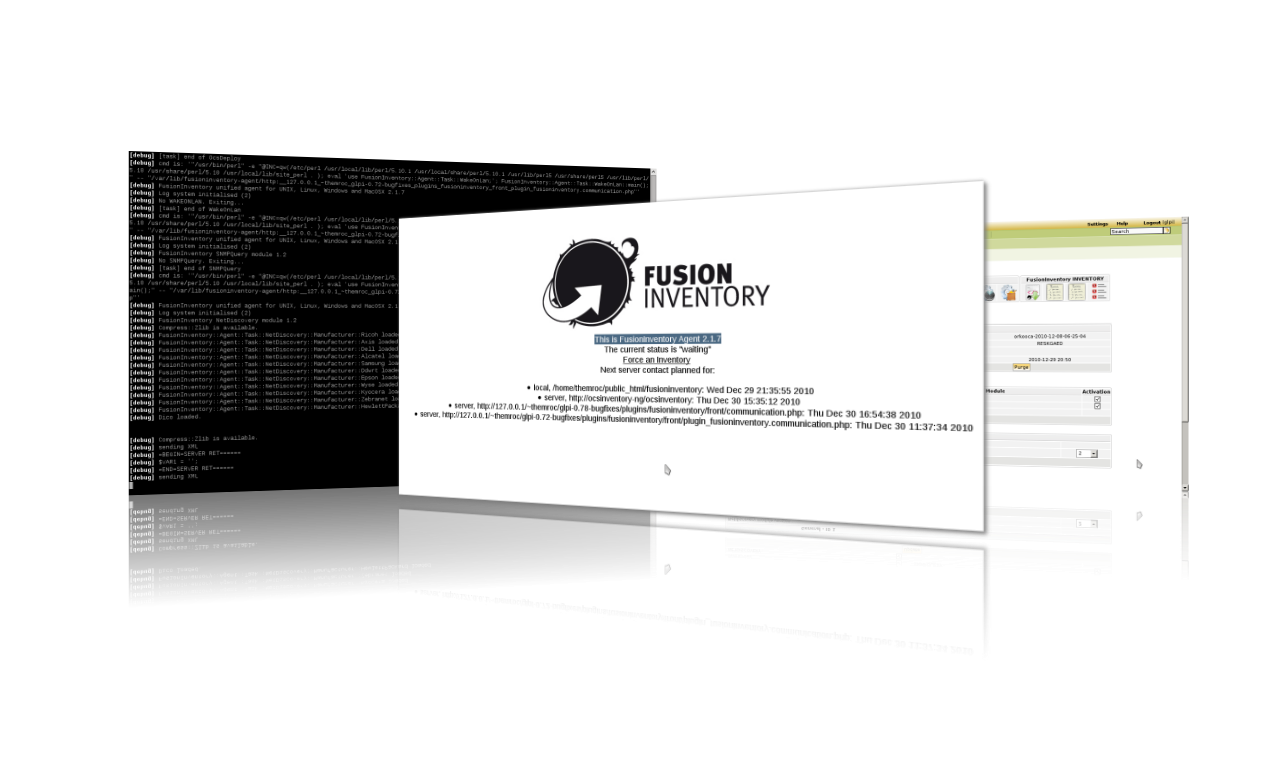
\includegraphics[height=4cm]{./pics/fusioninventory-tasks.png}}

\begin{frame}
\frametitle{Other tasks for the agent}
%
\begin{itemize}
%
\item wakeup
\item inventory on demand
\item wake on lan
\item peer to peer files transfert
\item custom tasks
%
\end{itemize}
\end{frame}
%-------------------------------------------------------------------
\subsection{LibFusionInventory}
%-------------------------------------------------------------------
\logo{
\includegraphics[height=1cm]{./pics/fusioninventory-logo.png}}

\begin{frame}
\frametitle{LibFusionInventory}

\begin{itemize}
%
\item PHP library
\item communication with agents
\item manage duplicate hardware
\item to integrate into another product
%
\end{itemize}
\end{frame}
%-------------------------------------------------------------------
\subsection{FusionInventory for GLPI}
%-------------------------------------------------------------------

\logo{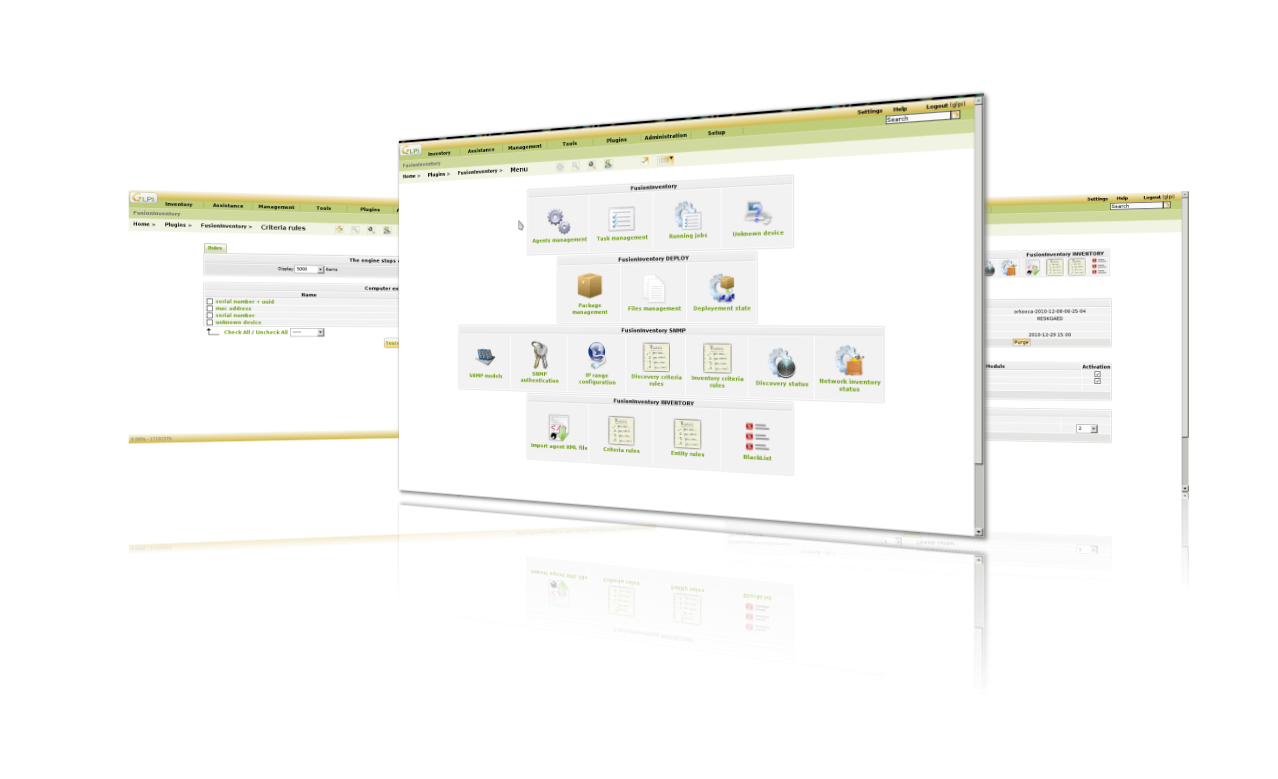
\includegraphics[height=3.5cm]{./pics/fusioninventory-glpi.png}}

\begin{frame}
\frametitle{FusionInventory for GLPI}

\begin{itemize}

\item inventory of computers, printers, switches
\item discover unknown hardware
\item planify tasks for agents
\item for GLPI 0.72 : released \\ without computers inventory
\item for GLPI 0.78 : beta in january

\end{itemize}
\end{frame}
%-------------------------------------------------------------------
\section{GLPI - Assets management}
%
%\logo{
\includegraphics[height=1cm]{./pics/glpi-logo.png}}
\logo{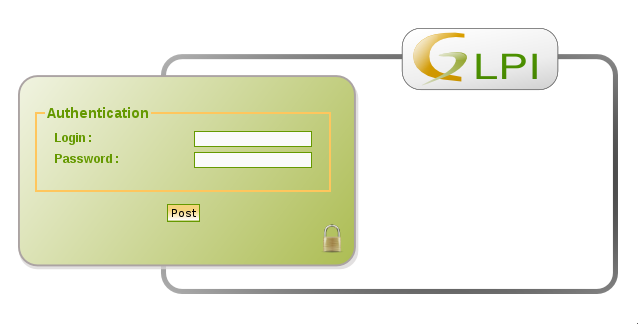
\includegraphics[height=2.5cm]{./pics/glpi-welcome.png}}

\subsection{GLPI facts - glpi-project.org}
%-------------------------------------------------------------------
\begin{frame}
\frametitle{GLPI facts - \href{http://glpi-project.org}{glpi-project.org}}
\logo{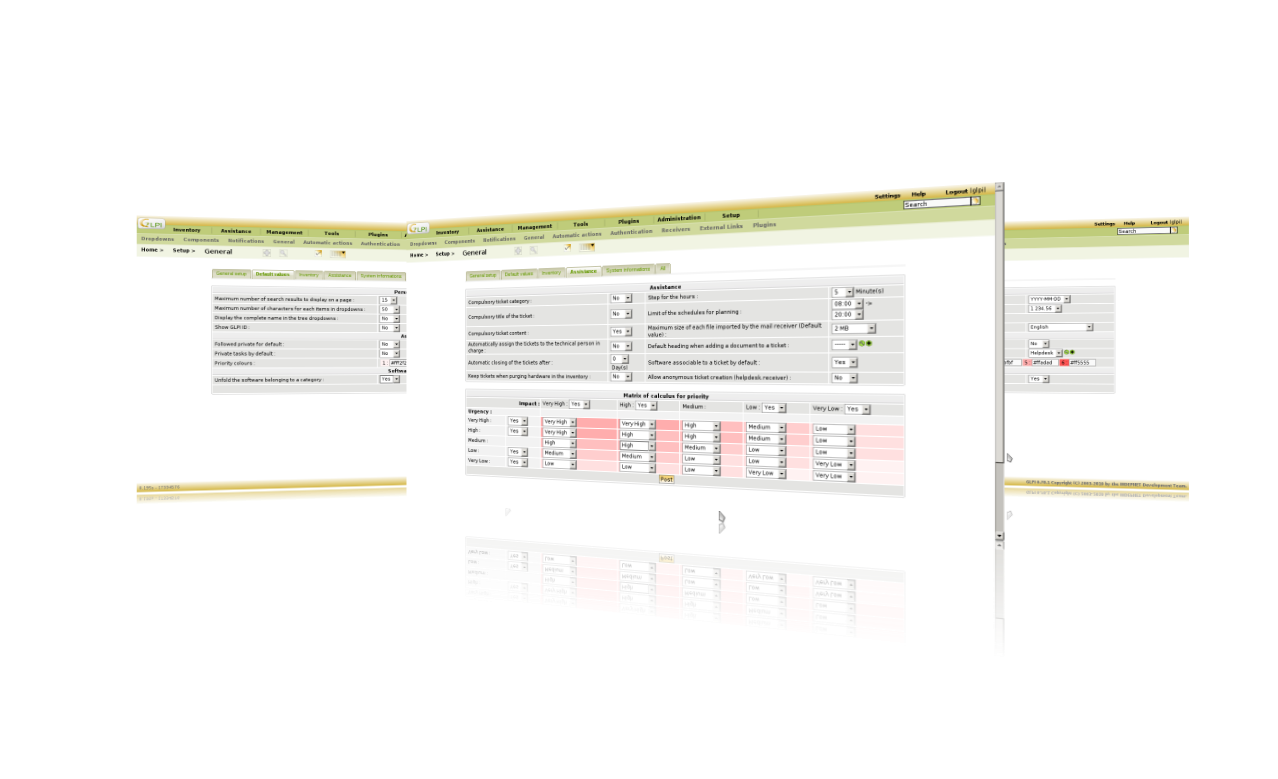
\includegraphics[height=3.5cm]{./pics/glpi-config.png}}
\begin{itemize}
%
\item GPLv2 PHP web application
\item IndepNet association, mainly french developers
\item worldwide usage, small to big business, administrations
\item authentication delegation (LDAP, IMAP, CAS)
\item strong separation of environments (entities)
\item i18n (35 languages)
\item data export
%
\end{itemize}
\end{frame}

%-------------------------------------------------------------------
\subsection{Assets inventory}
%-------------------------------------------------------------------
\logo{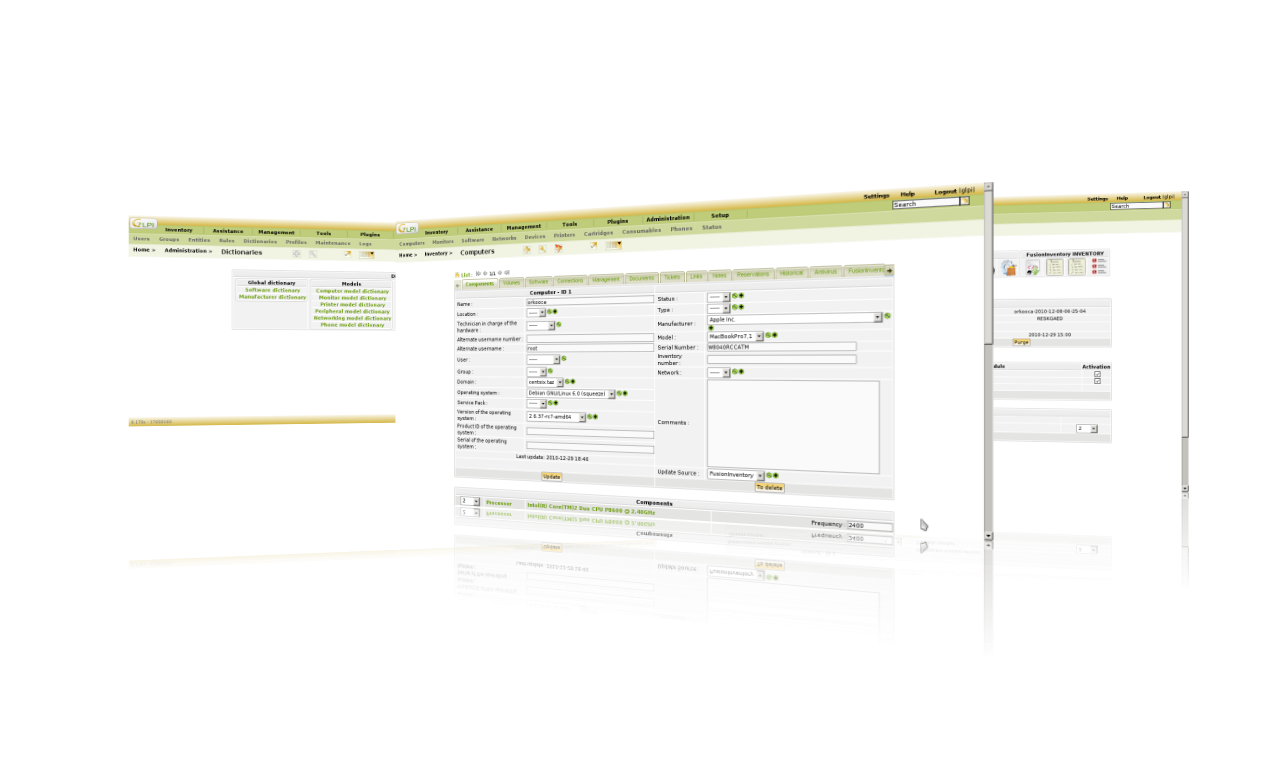
\includegraphics[height=3.5cm]{./pics/glpi-inventory.png}}

\begin{frame}
\frametitle{Assets inventory}

\begin{itemize}
%
\item data sources : OCSInventory-ng, FusionIventory server
\item importation, synchronization
\item normalisation with dictionaries
\item plugins for other sources
%
\end{itemize}
\end{frame}
%-------------------------------------------------------------------
\subsection{Helpdesk}
%-------------------------------------------------------------------
\logo{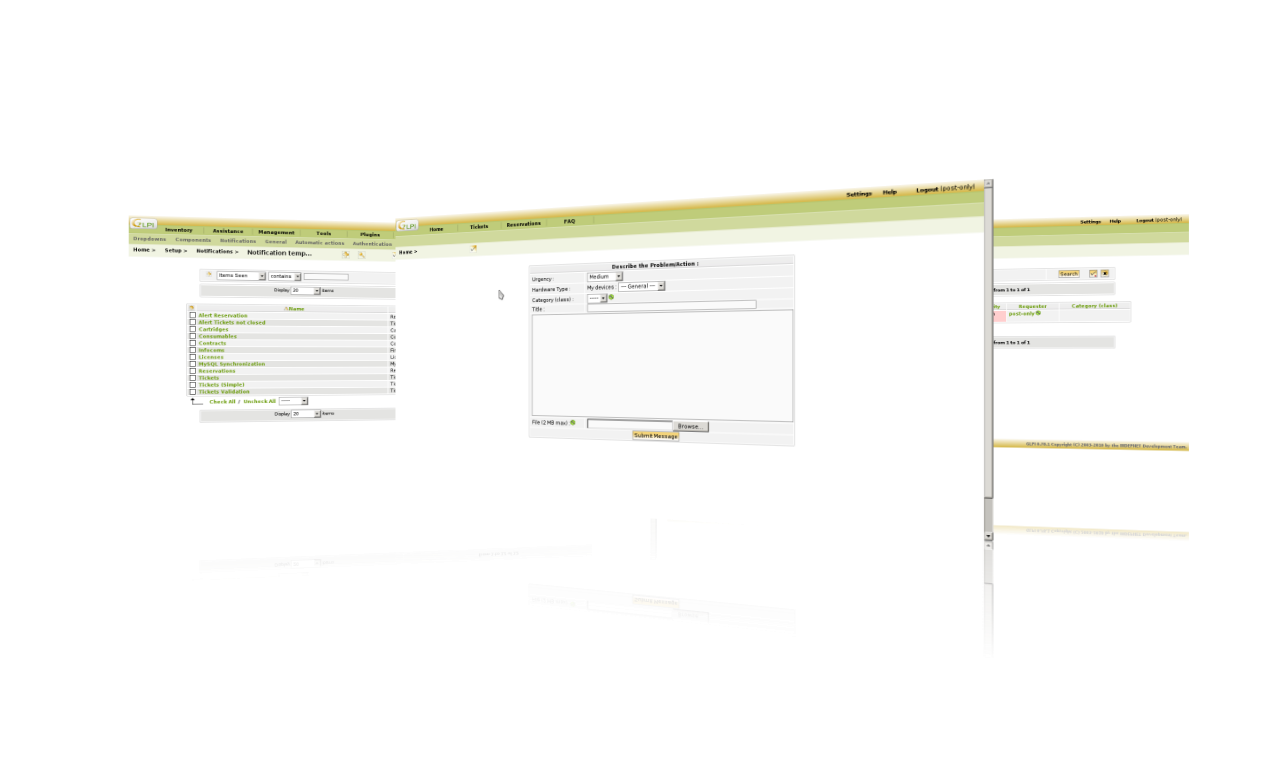
\includegraphics[height=3.5cm]{./pics/glpi-helpdesk.png}}
\begin{frame}
\frametitle{Helpdesk}
%
\begin{itemize}
%
\item simplified interface for helpdesk
\item ITIL compliance for incidents, service requests
\item business rules for tickets assignments
\item custom multilingual notifications
%
\end{itemize}
\end{frame}
%-------------------------------------------------------------------
\subsection{Useful Plugins}
%-------------------------------------------------------------------
\logo{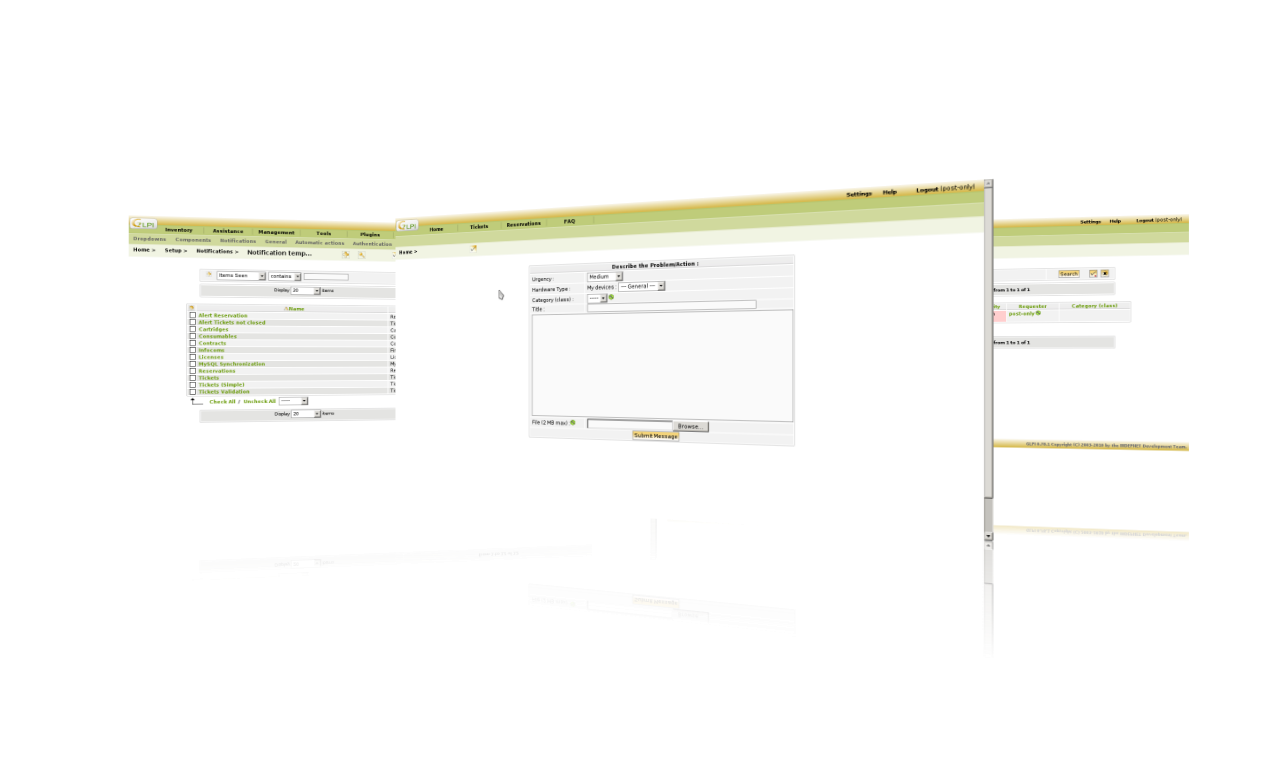
\includegraphics[height=3.5cm]{./pics/glpi-helpdesk.png}}
\begin{frame}
\frametitle{Useful Plugins}
%
\begin{itemize}
%
\item OCS Import (Automatic synchronization with OCS)
\item Manufacturers Import (Dell, HP, Fujistu-Siemens)
\item Accounts inventory (passwords keeper)
\item Data injection (CSV import)
\item Financial reports
\item PDF export
\item ...
%
\end{itemize}
\end{frame}
%

%-------------------------------------------------------------------
\subsection{New version : 0.78}
%-------------------------------------------------------------------
\logo{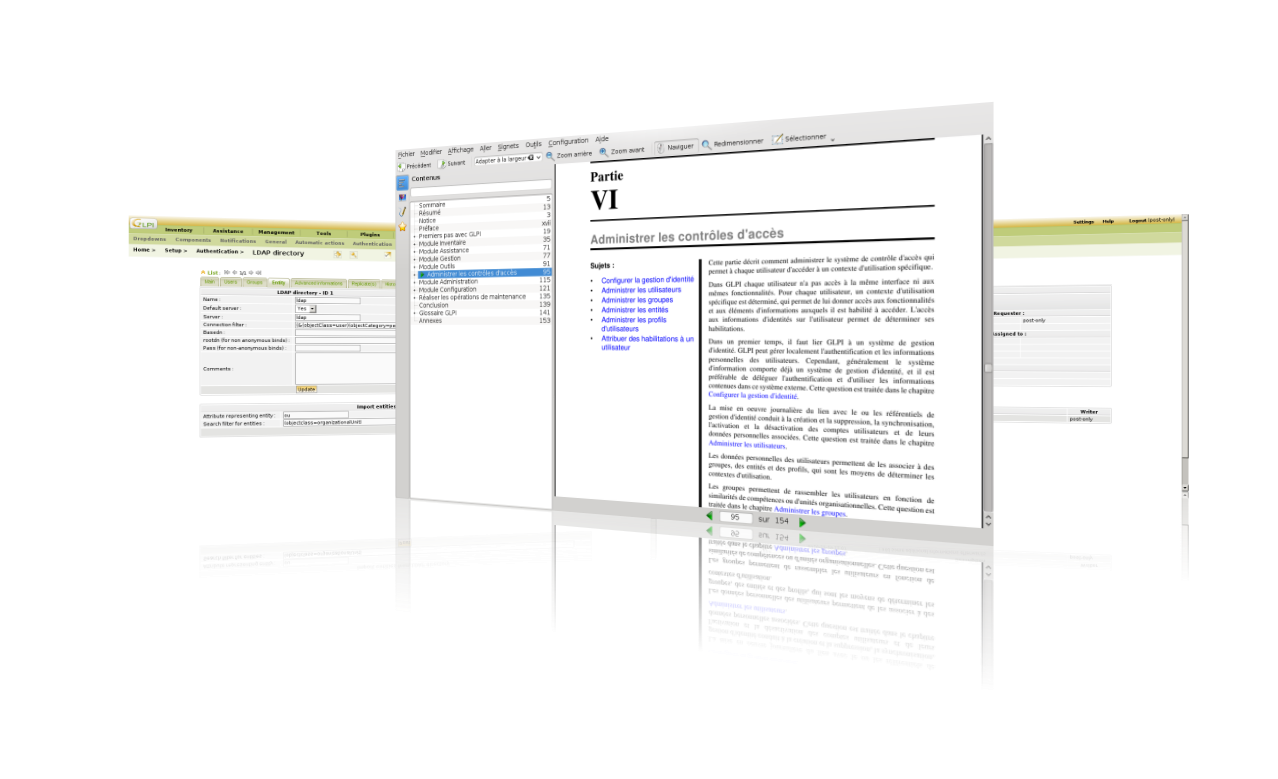
\includegraphics[height=3.5cm]{./pics/glpi-doc.png}}
%
\begin{frame}
\frametitle{Actual version : 0.78}
%
\begin{itemize}
%
\item entity based management enhanced (notifications, administrative closing, business rules, authentification)
\item helpdesk enhanced : tickets lifecycle, impact/urgency/priority matrix, ITIL
\item new database, framework, plugins API
\item LDAP enhancements
\item user interface polished
\item user documentation in french
%
\end{itemize}
\end{frame}
%-------------------------------------------------------------------
%\subsection{future}
%-------------------------------------------------------------------
%\logo{
\includegraphics[height=1cm]{./pics/glpi-logo.png}}
%\begin{frame}
%\frametitle{future}
%
%\begin{itemize}
%
%\item full ITIL v1 : SLA, user satisfaction
%\item helpdesk enhancements : links between tickets, links to KB, multiple assignments
%\item User documentation in english
%
%\end{itemize}
%
%\end{frame}
%-------------------------------------------------------------------

%\frame[plain]{}

\logo{
\includegraphics[height=1.5cm]{./pics/esquimaux-logo.png}}

\setbeamertemplate{headline}{
\includegraphics[width=\paperwidth, height=2cm, clip=true]{./pics/header.png}}
%\begin{frame}[plain]
\begin{frame}[shrink=20]{Outline}

\tableofcontents
%
\includegraphics[width=\columnwidth]{./pics/wolf.png} 
%\\
%
\includegraphics[height=1.5cm]{./pics/esquimaux-logo.png}

\end{frame}
\end{document}
